\documentclass[UTF8]{article}

\usepackage[zihao=5]{ctex}		%字号设置
\usepackage[a4paper]{geometry}	%页面设置
\geometry{left=2cm,right=2cm,top=2cm,bottom=5cm}

\usepackage{graphicx} 			%插入并编辑图片
\usepackage{siunitx}			%更好看的物理单位(手打其实更快些)
\usepackage{mhchem}				%写化学公式
\usepackage{chemfig}
\usepackage{fancyhdr}			%设置页眉页脚
\usepackage{lmodern}			%一种编码字体
\usepackage{amsmath}			%数学公式扩展
\usepackage{physics}

\usepackage{threeparttable}		%三线表宏包1
\usepackage{booktabs}			%三线表宏包2

\graphicspath{{figures/}}		%将报告中需要的图片储存于此

\pagestyle{fancy}				%设置页眉页脚
\setlength{\headheight}{70pt}
\lhead{
\includegraphics[scale=0.7]{logo}}
%需要将学校的logo名命并放入figures文件夹中
\chead{}
\rhead{}


\begin{document}				%开始文档

	\begin{center}
		\LARGE{\textbf{运算放大器}}

		\vspace*{0.2cm}
		\normalsize{戴佳乐 \quad PB18020556 \quad 苗立扬 \quad PB19000132}
	\end{center}
	\normalsize
	\section{实验目的}
	1. 掌握集成运放的基本特性和工作原理。
    
    2. 熟悉集成运放在模拟运算方面的应用。

	\section{实验原理}
    \subsection{集成运算放大器}
    集成运算放大器,是具有两个输入端、一个输出端的高增益、高输入阻抗的多级直接耦合放大电路。
    集成运算放大器的方框图如下

    \begin{figure}[htbp]
		\centering
        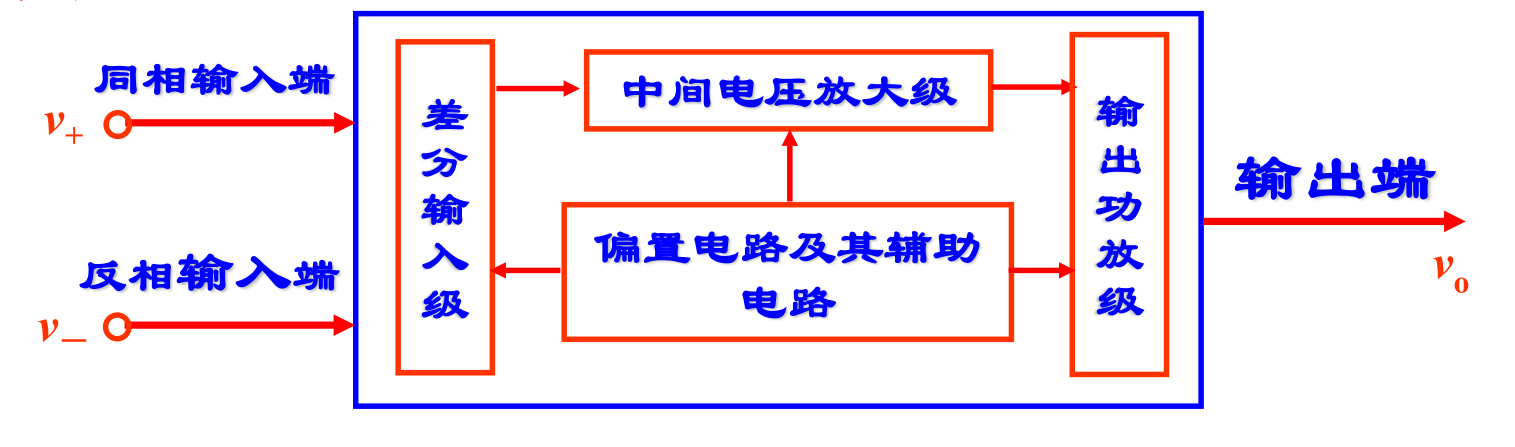
\includegraphics[width=0.8\linewidth]{sbbb0}
	\end{figure}

    输入级:高性能差放电路;输入电阻大、共模抑制比大、静态电流小。

中间级:复合管共射电压放大电路;提供电压放大。

输出级:互补对称输出电路。带载能力强、失真小。

偏置电路:电流源电路;提供合适的静态工作点。


	\subsection{反相比例运算电路}
    反相比例运算电路可以对反向后的输入信号进行比例运算,其原理图如图1所示

    \begin{figure}[htbp]
		\centering
        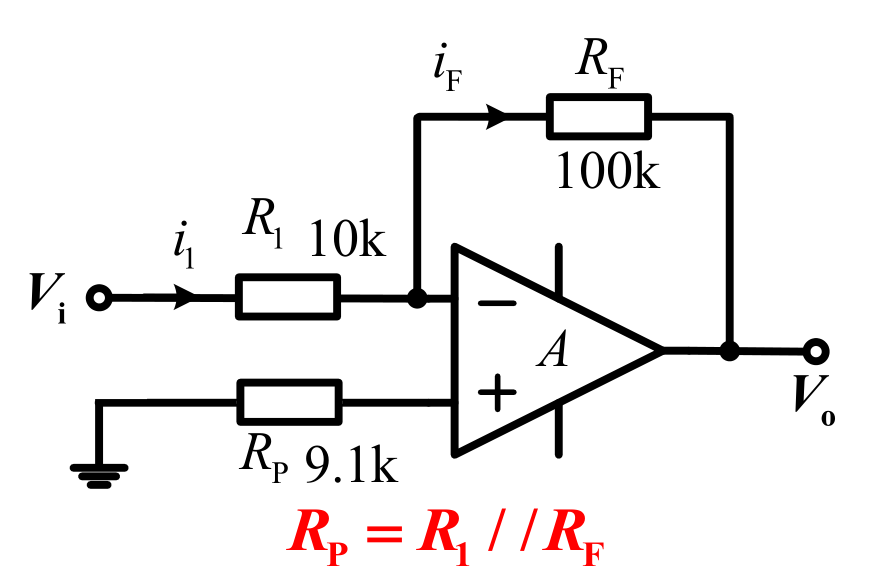
\includegraphics[width=0.5\linewidth]{sbbb1}
        \caption{反相比例运算电路}
	\end{figure}

    通过$R_F$引入负反馈,输出电压与输入电压反相并且比值受到反馈电阻和输入端$R_1$影响。
    输出电压和输入电压的关系为
    $$
    V_o=-\frac{R_F}{R_1} V_i
    $$

    \subsection{反相比例求和运算电路}
    原理图如图2所示

    \begin{figure}[htbp]
		\centering
        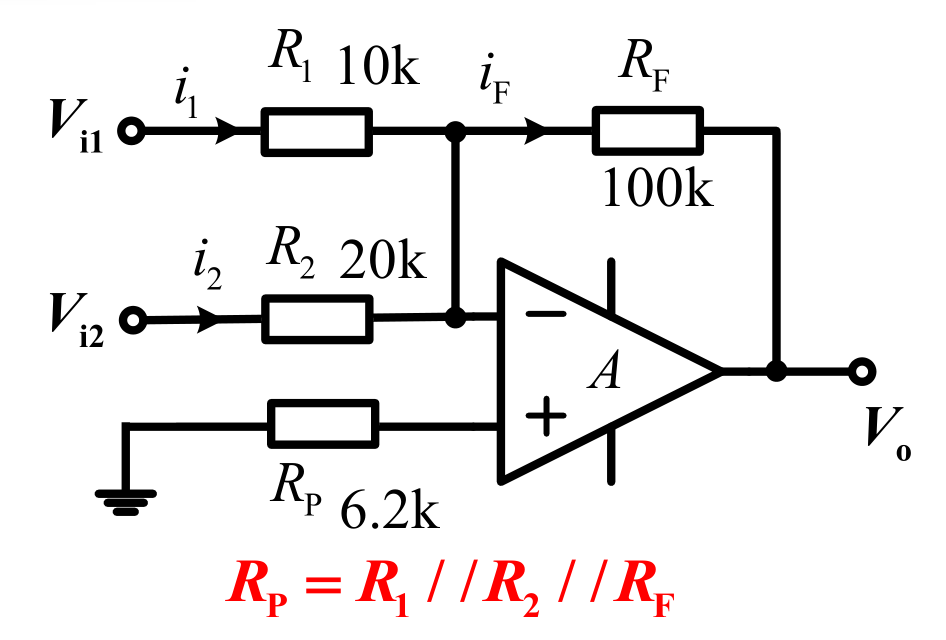
\includegraphics[width=0.5\linewidth]{sbbb2}
        \caption{反相比例求和运算电路}
	\end{figure}

    输出电压和输入电压的关系为
    $$
    V_o=-\frac{R_F}{R_1} V_{i1}-\frac{R_F}{R_2} V_{i2}
    $$

    \subsection{同相比例运算电路}
    原理图如图3所示

    \begin{figure}[htbp]
		\centering
        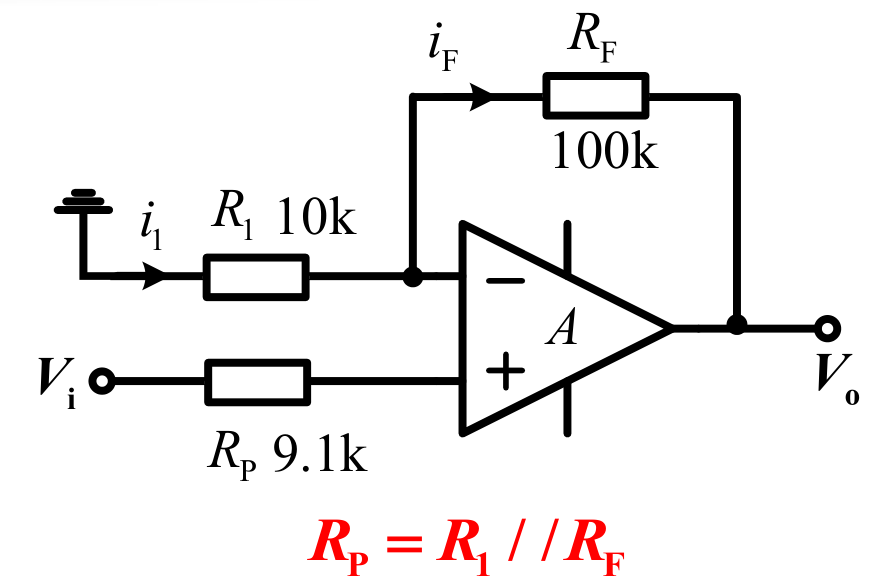
\includegraphics[width=0.5\linewidth]{sbbb3}
        \caption{同相比例运算电路}
	\end{figure}

    输出电压和输入电压的关系为
    $$
    V_o=\frac{R_F}{R_1} V_{i}+V_i
    $$

    \subsection{差动放大器}
    原理图如图4所示
    \begin{figure}[htbp]
		\centering
        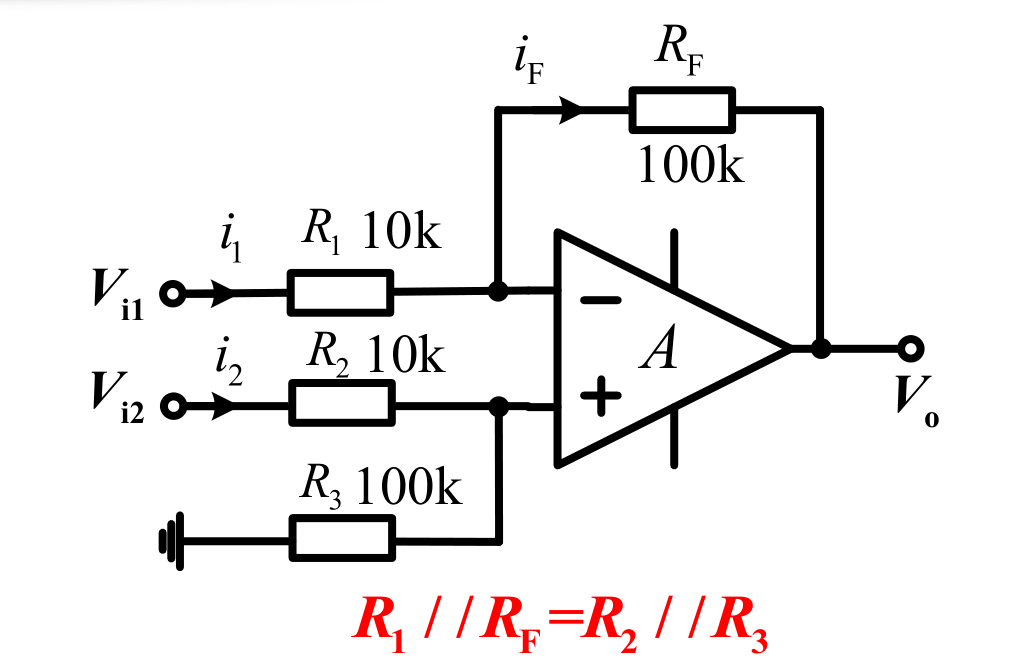
\includegraphics[width=0.5\linewidth]{sbbb4}
        \caption{差动放大器}
	\end{figure}

    输出电压和输入电压的关系为
    $$
    V_o=\frac{R_F}{R_1} \left(V_{i1}+V_{i2}\right)
    $$


    \subsection{积分电路}
    原理图如图5所示

    \begin{figure}[htbp]
		\centering
        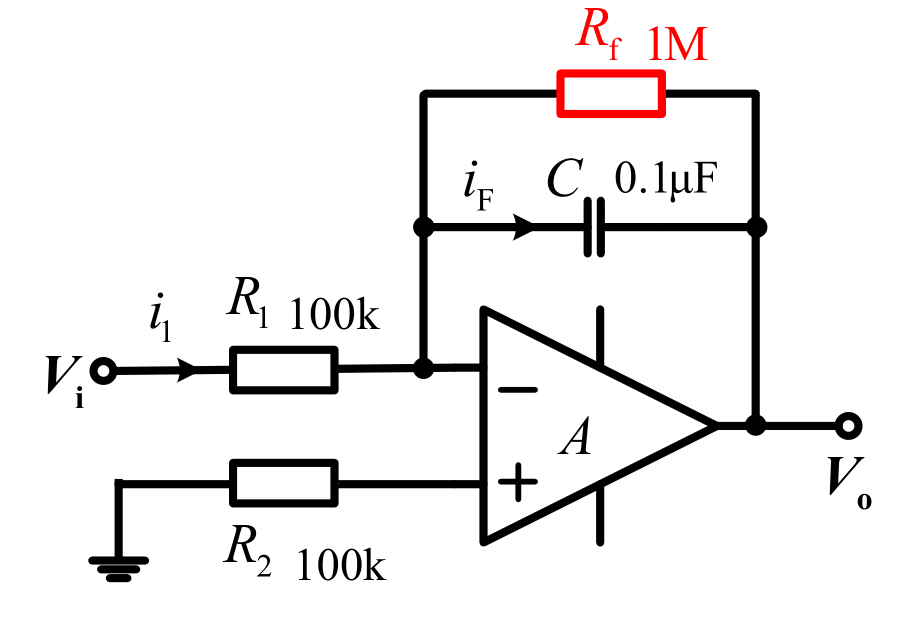
\includegraphics[width=0.5\linewidth]{sbbb5}
        \caption{积分电路}
	\end{figure}

    对输出信号 $V_{o}$ 有
    $$
    V_{o}=-V_{c}=-\frac{1}{R_{1} C} \int_{0}^{t_{1}} u_{i} \mathrm{~d} t+V_{c}(0)
    $$
    
    \subsection{微分电路}
    原理图如图6所示

    \begin{figure}[htbp]
		\centering
        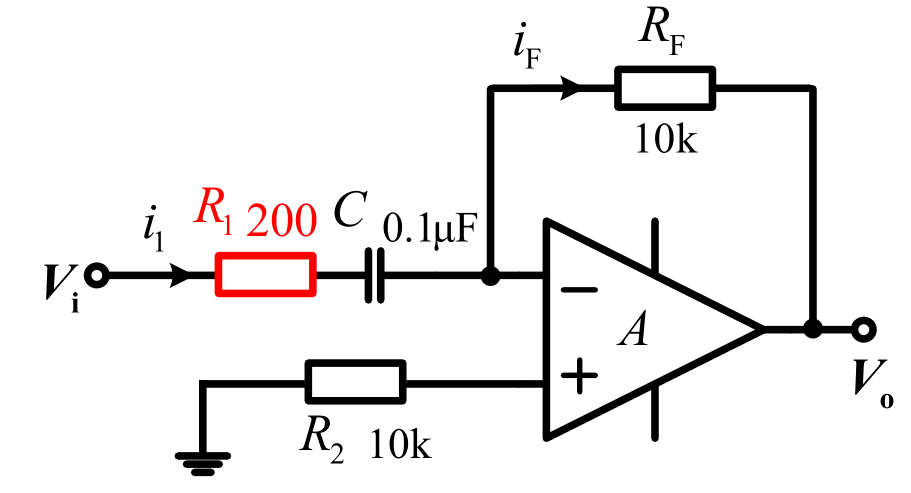
\includegraphics[width=0.5\linewidth]{sbbb6}
        \caption{微分电路}
	\end{figure}

    输出电压
    $$
    V_o = - R_F C \frac{\dd V_i}{\dd t}
    $$





    \section{LM324型集成电路}
    LM324是四运放集成电路,它采用14脚双列直插塑料封
装,示意图如图7所示。它的内部包含四组形式完全相同
的运算放大器,除电源共用外,四组运放相互独立。

\begin{figure}[htbp]
    \centering
    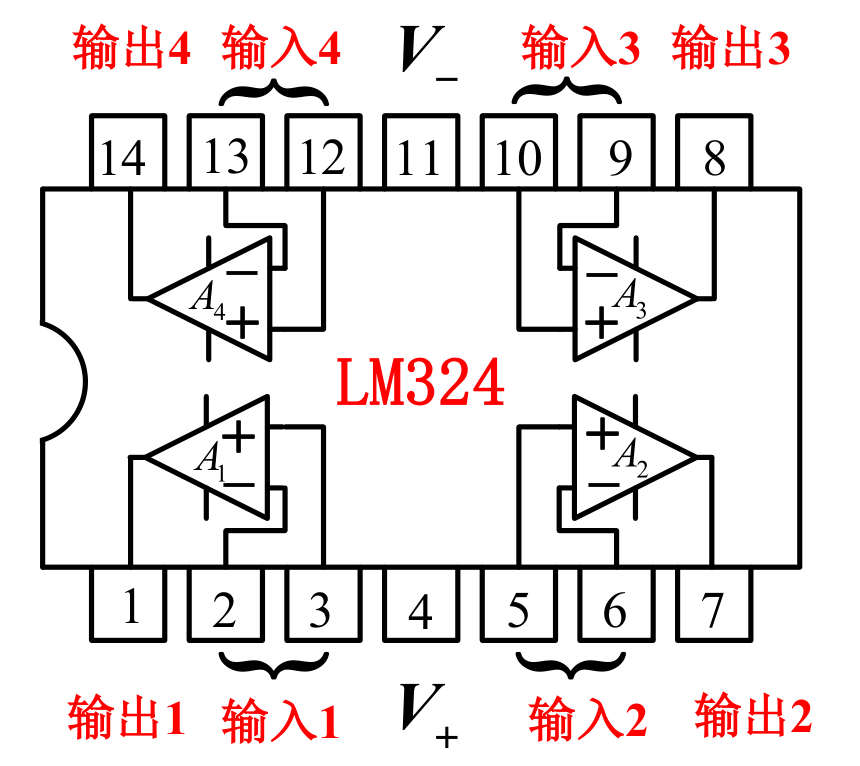
\includegraphics[width=0.3\linewidth]{sbbb7}
    \caption{LM324集成电路示意图}
    
\end{figure}

\section{实验数据与数据分析}
\subsection{反相比例运算电路}
\subsubsection{反相比例运算电路 实验数据}
实验数据如表1所示:
% Table generated by Excel2LaTeX from sheet 'Sheet1'
\begin{table}[htbp]
	\centering
	\caption{反向比例运算电路实验数据}
	\begin{tabular}{|r|r|r|r|}
		\toprule
		\multicolumn{1}{|l|}{$V_i$} & \multicolumn{1}{l|}{$V_o$} & \multicolumn{1}{l|}{$A_v(实测)$} & \multicolumn{1}{l|}{$A_v(理论)$} \\
		\midrule
		0.1678 & 1.649 & -9.83 & -10 \\
		\bottomrule
	\end{tabular}%
	\label{tab1}%
\end{table}%
实验所得的$U_i$图与$U_o$图在示波器上的图像如实验报告纸所示。

\subsubsection{反相比例运算电路 数据分析}
从实验中我们看到,反相电路的输出波形与输入波形波形大致相反,信号幅度显著放大,初步验证了该运算放大电路的作用。与此同时,通过对理论值与实验实际测量的放大倍数的对比,我们得出误差为
$$\delta = |\frac{-9.83+10}{10}|\times 100\% = 1.7\% $$
实验值与理论值吻合得很好。
	
	
\subsection{反相比例求和运算电路}
\subsubsection{反相比例求和运算电路 实验数据}
实验数据如表2所示:
% Table generated by Excel2LaTeX from sheet 'Sheet1'
\begin{table}[htbp]
	\centering
	\caption{反相比例求和运算电路 实验数据}
	\begin{tabular}{|l|r|r|r|r|r|r|}
		\toprule
		$V_{i1}$ & 0.28271 & 0.38074 & 0.47918 & -0.2813 & -0.38014 & -0.47906 \\
		\midrule
		$V_{i2}$ & 0.42847 & 0.62612 & 1.02623 & -0.4276 & -0.62594 & -1.02623 \\
		\midrule
		$V_{o}$ & -4.8974 & -6.8499 & -9.4415 & 4.9358 & 6.9007 & 9.8719 \\
		\midrule
		$V_{o}理论$ & -4.9695 & -6.938 & -9.9229 & 4.951 & 6.9311 & 9.9218 \\
		\bottomrule
	\end{tabular}%
	\label{tab2}%
\end{table}%
\subsubsection{反相比例求和运算电路 数据分析}
将测量得到的输出实际值与理论值对比,我们的误差最大不超过$|\frac{9.4415-9.9229}{9.9229}| = 4\% $。考虑可能存在的电阻值误差与测量误差,我们得出结论,我们较好地验证了反向比例求和运算电路的关系式

\subsection{同相比例运算电路}
\subsubsection{同相比例运算电路 实验数据}
实验数据如表3所示:
% Table generated by Excel2LaTeX from sheet 'Sheet1'
% Table generated by Excel2LaTeX from sheet 'Sheet1'
\begin{table}[htbp]
	\centering
	\caption{同相比例运算电路 实验数据}
	\begin{tabular}{|r|r|r|r|}
		\toprule
		\multicolumn{1}{|l|}{$V_i$} & \multicolumn{1}{l|}{$V_o$} & \multicolumn{1}{l|}{$A_v(实测)$} & \multicolumn{1}{l|}{$A_v(理论)$} \\
		\midrule
		0.1682 & 1.82  & 10.82 & 11 \\
		\bottomrule
	\end{tabular}%
	\label{tab:addlabel}%
\end{table}%

实验所得的$U_i$图与$U_o$图在示波器上的图像如实验报告纸所示。

\subsubsection{同相比例运算电路 数据分析}
从实验中我们看到,同相电路的输出波形与输入波形波形大致相同,信号幅度显著放大,初步验证了该运算放大电路的作用。与此同时,通过对理论值与实验实际测量的放大倍数的对比,我们得出误差为
$$\delta = |\frac{11-10.82}{11}|\times 100\% = 1.6\% $$
实验值与理论值吻合得很好。

\subsection{差动放大电路}
\subsubsection{差动放大电路 实验数据}
实验数据如表2所示:
% Table generated by Excel2LaTeX from sheet 'Sheet1'
\begin{table}[htbp]
	\centering
	\caption{差动放大电路 实验数据}
	\begin{tabular}{|l|r|r|r|r|r|r|}
		\toprule
		$V_{i1}$ & 0.18281 & 0.47861 & 0.67627 & -0.18261 & -0.47855 & -67617 \\
		\midrule
		$V_{i2}$ & 0.52688 & 0.82376 & 1.0259 & -0.52675 & -0.8237 & -1.0258 \\
		\midrule
		$V_{o}$ & 3.4222 & 3.4317 & 3.4733 & -3.3853 & -3.3949 & -3.38 \\
		\midrule
		$V_{o}理论$ & 3.4407 & 3.4515 & 3.4963 & -3.4414 & -3.4515 & -3.4963 \\
		\bottomrule
	\end{tabular}%
	\label{tab5}%
\end{table}%

\subsubsection{差动放大电路 数据分析}
将测量得到的输出实际值与理论值对比,我们的误差最大不超过$|\frac{3.380-3.4963}{3.4963}| = 3\% $。考虑可能存在的电阻值误差与测量误差,我们得出结论,我们较好地验证了差动放大电路的关系式

\subsection{积分电路}
搭载电路如图5所示。接入方波后,输出电压的交流电成分为近似的三角波,与实验分析的结果一致,其中三角波斜率与电压的关系符合理论分析的结果,为$-\frac{U}{RC} = 0.5$,与实验测得的0.5相近。

通过该波形,我们较好验证了积分电路的波形与输入电压的积分关系。


\subsection{微分电路}
搭载电路如图6所示。接入三角波后,输出电压的交流电成分为近似的方波,与实验分析的结果一致,其中方波大小与电压的关系符合理论分析的结果,为$-\frac{U}{RC} \times 4 = 8$,与实验测得的8.625相近。

通过该波形,我们较好验证了微分电路的波形与输入电压的积分关系。

\section{思考题}
	\subsection{如何判断集成运算放大器的好坏?为了不损坏集成运算放大器,实验中应注意什么问题?}
	良好的集成运放符合虚短与虚断的性质。测量集成运放两输入端的电压,若电压相同,电流很小,说明集成运放工作在正常工作区且无损坏。反之,说明运放出现了故障,有PN结被击穿损坏。
	
	为了不损坏集成运放,实验中需要注意接入电源的极性与电压的大小,避免PN结在过高偏置下被击穿失去功能。
	
	\subsection{在反相比例求和电路图7-2中,如果Vi1和Vi2均采用直流信号,并选定Vi2=-1V,考虑到运算放大器的最大输出幅度为±12V,Vi1的绝对值不应超过多少伏?}
	考虑输出与输入电压的关系为
	 $$
	V_o=-\frac{R_F}{R_1} V_{i1}-\frac{R_F}{R_2} V_{i2} = -10V_{i1}-5V_{i2}
	$$
	$V_{i1}$最大为+1.7V,最小为0.7V
	
	所以$V_{i1}$的绝对值不超过1.7V
	
	\subsection{设计两个能实现下列运算关系的运算电路。}
	
	\subsubsection{$V_{\mathrm{o}}=2 V_{11}+2 V_{12}-4 V_{13}$}
	将$V_{11}$与$V_{12}$接入反相求和运算电路,设置$R_1 = 100k \Omega$,$R_2 = 100k \Omega$, $R_F = 200k \Omega$,$R_P = 40k \Omega$得到-2$V_{12}$-2$V_{11}$。随后将该电压与$V_{13}$接入另一反相比例放大器,设置$R_1 = 100k \Omega$,$R_2 = 25k \Omega$, $R_F = 100k \Omega$,$R_P = 17k \Omega$,得到所需电压。
	
	\subsubsection{$V_{o}=2 V_{11}-3 V_{12}$}
	将$V_{11}$接入反相比例运算电路,设置$R_1 = 10k \Omega$,$R_F = 20k \Omega$, $R_P = 6.7k \Omega$得到-2$V_{11}$,再将-2$V_{11}$与$V_{12}$接入反相求和电路,设置$R_1 = 100k \Omega$,$R_2 = 33k \Omega$, $R_F = 100k \Omega$,$R_P = 19.8k \Omega$,此时反向求和运放得到的就是我们所需的电压。
	
\end{document}